\documentclass{beamer}
\usetheme{Dresden}
%\setbeameroption{show notes}

\setbeamercovered{transparent}

\usepackage[utf8x]{inputenc}
\usepackage{amsmath}
\usepackage{amssymb}
\usepackage{amsfonts}
\usepackage{amsthm}
\usepackage{ucs}
\usepackage{cite}
\usepackage{stmaryrd}
\usepackage{hyperref}
\usepackage{xifthen}
\usepackage{graphicx}
\usepackage{syntax}
\usepackage{xspace}
\usepackage{algorithm}
\usepackage[noend]{algpseudocode}
\usepackage{listings}

\lstnewenvironment{code}{\lstset{language=Haskell,basicstyle=\small}}{}

\newcommand*{\pfunc}{\xrightarrow{p}}
\newcommand*{\peq}{\simeq}
\newcommand*{\listOf}[1]{\left< #1 \right> }
\newcommand*{\coded}[1]{\ulcorner #1 \urcorner }
\newcommand*{\turingletter}[1]{\left< #1 \right> }
\newcommand*{\WHILE}{\ensuremath{\mathtt{WHILE}}\xspace}
\newcommand*{\FOR}{\ensuremath{\mathtt{FOR}}\xspace}
\newcommand*{\TM}{\ensuremath{\mathtt{TM}}\xspace}
\newcommand*{\N}{\ensuremath{\mathbb{N}}\xspace}
\newcommand{\lepower}{\leq}
\newcommand{\gepower}{\geq}
\newcommand{\epower}{\equiv}
\newcommand{\abs}[1]{\left|#1\right|}
\newcommand{\TIME}[1][]{\mathtt{TIME}\ifthenelse{\isempty{#1}}{}{_{#1}}}
\newcommand{\SPACE}[1][]{\mathtt{SPACE}\ifthenelse{\isempty{#1}}{}{_{#1}}}
\newcommand{\LOGTIME}{\mathtt{LOGTIME}}
\newcommand{\LOGSPACE}{\mathtt{LOGSPACE}}
\newcommand{\PTIME}{\mathtt{PTIME}}
\newcommand{\PSPACE}{\mathtt{PSPACE}}
\newcommand{\EXPTIME}{\mathtt{EXPTIME}}
\newcommand{\EXPSPACE}{\mathtt{EXPSPACE}}
\mathchardef\mhyphen="2D

% Note Commands
\newcommand{\citationneeded}{\alert{(citation needed) } }
\newcommand{\lineofthought}[1]{{\bf [#1] }}
\newcommand{\TODO}{\ensuremath{\left<\mathbf{TODO}\right> }}

% Disabled Note Commands
\newcommand{\timeestimation}[1]{}
%\newcommand{\citationneeded}{}
%\newcommand{\lineofthought}[1]{}
%\newcommand{\TODO}{}

\newcommand{\interpret}[2][]{\ensuremath{\left\llbracket #2 \right\rrbracket
	\ifthenelse{\isempty{#1}}{}{_{#1}}}}
\newcommand{\Input}[1][]{\ensuremath{I
	\ifthenelse{\isempty{#1}}{}{_{#1}}}}
\newcommand{\Output}[1][]{\ensuremath{O
	\ifthenelse{\isempty{#1}}{}{_{#1}}}}
\newcommand{\Compiler}[3][]{\ensuremath{compile_{#2\rightarrow #3}
	\ifthenelse{\isempty{#1}}{}{^{#1}}}}
\newcommand{\Interpreter}[2][]{\ensuremath{interpret_{#2}
	\ifthenelse{\isempty{#1}}{}{^{#1}}}}
\newcommand{\measuretime}[2][]{\ensuremath{T_#2
	\ifthenelse{\isempty{#1}}{}{^{#1}}}}
\newcommand{\measurespace}[2][]{\ensuremath{S_#2
	\ifthenelse{\isempty{#1}}{}{^{#1}}}}
\newtheorem{prop}{Proposition}
\newtheorem{corrolary}{Corrolary}
\newtheorem{thesis}{Thesis}
\theoremstyle{definition}
\newtheorem{defn}{Definition}

\author{Aaron Karper}
\title{A Programming Language Oriented Approach to Computability}
\institute{Institute of Computer Science and Applied Mathematics\\ Universität Bern}
\date{2012}
\AtBeginSection[]{
  \begin{frame}<beamer>
    \frametitle{Outline for section \thesection}
    \tableofcontents[currentsection, hideothersubsections]
  \end{frame}
}
\begin{document}

\frame{\maketitle}
\frame{\tableofcontents}

\section{Introduction}
\subsection{Goal}
\frame{
	\frametitle{Goal}
	\begin{itemize}[<+->]
		\item Introduction to methods and theorems of computability and 
			complexity \note{Focus is however on computability}
		\item To be read in parallel to the Computability and Complexity Lecture 
			by Prof. Strahm
		\item Connect theory and practical application\note{practical application 
				reach from JIT compilers that use partial evaluation, how 
				applications are ported to new architectures and how we can formulate 
				Churches thesis so that it can be checked scientifically.}
		\item With a formalism easily understandable by students in the fourth semester
			\note{Means that prerequisites should be very low -- no formal logic, few
			data structures, only scratching formal languages. Basically, the text 
			should be self contained}
	\end{itemize}
}

\subsection{Some Definitions}
\begin{frame}{Semantic Function}
	\note{Semantic functions are used in a style of defining languages called
		{\em denotational semantics}. It gives very precise specifications for a
		language, but for complex languages, it is nigh impossible to write them
		down.}
	\pause
	The \alert{semantic function}\/ translates between the language $L$, we use to 
	describe a program and the mathematical objects $M$, it describes.

	\pause
	For example:
	\begin{equation*}
		\interpret[\lambda \text{-calculus}]{\lambda x.\,x}(f) = id(f) = f
	\end{equation*}
	\pause
	If given explicitly it gives a specification for the programming language.
	\pause

	The value $\bot$ denotes that an interpretation does not exists, i.e.\ that 
	an expression is an error or does not terminate.
\end{frame}

\begin{frame}[fragile]{The {\tt Cons}\/ cell data structure}
	\note{This is like in LISP, the cons cell is very flexible and incorporates 
	pointers, that could allow sub-linear runtimes.}
	\begin{center}
		\begin{code}
			data Cons = Nil | ConsCell { hd :: Cons, tl :: Cons }
		\end{code}
		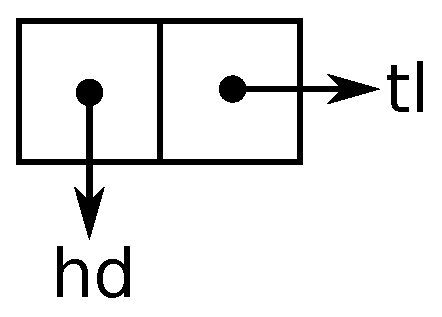
\includegraphics[width=0.25\textwidth]{pictures/conscell}
	\end{center}
	The {\tt cons}\/ cell is a simple data structure that contains a head and a 
	tail pointer. We denote this by {\tt (h.t)}\/ where {\tt h}\/ is the head and 
	{\tt t}\/ is the tail.
	\pause

	Used to build simply linked lists, binary trees, \dots
\end{frame}

\subsection{\WHILE}
\begin{frame}[fragile]{The \WHILE programming language}
	A basic, imperative, Turing-complete languages, using {\tt cons} cells to 
	represent data.
	
	\note{\begin{itemize}
		\item Very basic, but Turing complete language.
		\item Imperative
		\item Uses the {\tt cons} cell as basic data structure.
	\end{itemize}}
	\begin{example}
		\begin{verbatim}
unary_minus_one read X {
  if X {
    X := tl X;
  }
} write X\end{verbatim}
	\end{example}
\end{frame}

\begin{frame}[fragile]{The \WHILE programming language -- Syntax}
	\note{\begin{description}
			\item[Expressions] nil, cons of two exps, hd or tl of an exp and 
				variables. Symbols for added convenience. Functions also, but will 
				not go into details.
			\item[Statements] Assignment, while -- for and if for convenience
			\item[Procedures] 
		\end{description}}
	\begin{center}
		\begin{tiny}
			\begin{grammar}
				<expression> ::= 
									`nil' 
						\alt 	`cons' <expression> <expression>
						\alt 	`hd' <expression>
						\alt 	`tl' <expression>
						\alt 	<variable>
						\alt 	`:' <name>

				<statement-list> ::= <statement> ; \alt <statement> ; <statement-list>

				<block> ::= `{' <statement-list> `}'

				<statement> ::=
									<variable> `:=' <expression>
						\alt	`if' <expression> <block> <else-block>
						\alt	`while' <expression> <block>
						\alt	`for' <variable> `in' <expression> <block>
					
						<else-block> ::= <empty> \alt `else' <block>
						
						<program> ::= <name> `read' <variable> <block> `write' <variable>
			\end{grammar}
		\end{tiny}
	\end{center}
\end{frame}

\begin{frame}[fragile]{The \WHILE programming language -- Semantics}
	
	The data expressions might depend on the context $c$, which binds variable 
	names to their values.

	\begin{small}
		\begin{align*}
			\interpret{\mathtt{nil}}(c) &= Nil \\
			\interpret{\mathtt{cons}\: A\: B}(c) &= ConsCell(\interpret{A}(c), \interpret{B}(c)) \\
			\interpret{\mathtt{hd}\: A}(c) &= \begin{cases}
				x, &\text{ if }\interpret{A}(c) = ConsCell(x, y)\\
				\bot, &\text{ otherwise}
			\end{cases}\\
			\interpret{\mathtt{tl}\: A}(c) &= \begin{cases}
				y, &\text{ if }\interpret{A}(c) = ConsCell(x, y)\\
				\bot, &\text{ otherwise}
			\end{cases}\\
			\interpret{name}(c) &= \begin{cases}
				x, &\text{ if } (name, x) \in c\\
				Nil, &\text{ otherwise}
			\end{cases}
		\end{align*}
	\end{small}
\end{frame}

\begin{frame}{The \WHILE programming language -- Semantics}
	The statements change the context, so their interpretation returns the new context.
	\begin{align*}
		\interpret{name\: := a}(c) &= (c\setminus \{(name, x)\}) \cup (name, \interpret{a}(c)) \\
		\interpret{\mathtt{if}\: a\: block}(c) &= \begin{cases}
			c, &\text{ if }\interpret{a}(c)= Nil\\
			\interpret{block}(c), &\text{ otherwise}
		\end{cases}\\
		\interpret{\mathtt{while}\: a\: b}(c) &= \begin{cases}
			c, &\text{ if }\interpret{a}(c) = Nil\\
			(\interpret{\mathtt{while}\: a\: b}\circ\interpret{b})(c), &\text{ otherwise}
		\end{cases}
	\end{align*}
\end{frame}

\begin{frame}{The \WHILE programming language -- Semantics}
	The programs represent functions:

	\begin{align*}
		\interpret{a\: \mathtt{read}\: i\: block \: \mathtt{write}\: o}(x) &= 
		(\interpret{o}\circ\interpret{block})(\{(i, x)\})
	\end{align*}

	For the rest of the presentation, we only interpret programs.
\end{frame}

\section{Transforms}
\subsection{Programs acting on programs}
\begin{frame}{Programs acting on programs}
	In any programming language $A$ we define:
	\begin{description}
		\item[interpreter] An \alert{interpreter}\/ for a language $L$ is a program $interpret$, such 
			that \[\forall p\in L: \interpret[A]{interpret}(p,x) =\interpret[L]{p}(x)\]
			\note{This is analogous to giving an implementation of the semantic function}
		\item[compiler] A \alert{compiler}\/ for a language $L$ is a program $compile$, 
			such that 
			\[\forall p\in L: \interpret[A]{\interpret[A]{compile}(p)}(x)= \interpret[L]{p}(x)\]
		\item[specializer] A \alert{specializer}\/ is a program $spec$, such that 
			\[\forall p\in A: \interpret[A]{\interpret[A]{spec}(p, x)}(y) = \interpret[A]{p}(x, y)\]
	\end{description}
\end{frame}

\begin{frame}{Comparing Programming Languages}
	A language $A$ is \alert{at least as strong} as $B$, written $B\lepower A$, if there is a 
	\alert{compiler} written in $A$ for $B$. 
	\begin{example}
		\begin{itemize}[<+->]
			\item \WHILE is at least as strong as Turing machines and vice versa.
			\item {\tt Haskell}  is at least as strong as \WHILE.
			\item \WHILE is at least as strong as {\tt 3-SAT}.
			\item {\tt 3-SAT} is at least as strong as any other problem in {\tt NP-TIME}.
		\end{itemize}
	\end{example}
\end{frame}

\subsection{Futamura Projections}
\begin{frame}{Futamura Projections}
	\begin{itemize}[<+->]
		\item Interpreters are easy to write, but slow. Compilers on the other 
			hand give fast programs, but are hard to write.
		\item Specializers are often used, to create faster executables, because 
			static analysis can optimize the procedures used.
		\item The \alert{Futamura projections} show how executable programs,
			interpreters and compilers are connected, if we assume a specializer.
	\end{itemize}
\end{frame}

\begin{frame}{The first Futamura Projection}
	Given a program $p$ in a language $L$, can we make it an executable in $A$?
	\pause

	\invisible<1>{ 
		Yes, $\interpret{spec}(interpret, p)$ is such a program:
		\begin{align*}
			\interpret[A]{\interpret[A]{spec}(interpret, p)}(x) 
					&= \interpret[A]{interpret}(p, x)\\
					&= \interpret[L]{p}(x)
		\end{align*}
	}
\end{frame}

\begin{frame}{The first Futamura Projection}
	But is this useful?

	\pause
	\begin{itemize}
		\item Many interpreted languages have libraries, that bundle the 
			interpreter and the used libraries with the source code.
			\begin{itemize}
				\item {\tt bbfreeze} for {\tt Python}
				\item {\tt releasy} for {\tt Ruby}
				\item \dots
			\end{itemize}
		\item Specializer is here on the OS level, bundling libraries and executables.
	\end{itemize}
\end{frame}

\begin{frame}{The second Futamura Projection}
	Do we need to write a compiler for $L$, if we already have an interpreter?
	\pause

	\invisible<1>{
		No, we can modify the first projection, then 
		$compile = \interpret{spec}(spec, interpret)$
		\begin{align*}
			\interpret[A]{\interpret[A]{\interpret[A]{spec}(spec, interpret)}(p)}(x)\\
			&= \interpret[A]{\interpret{spec}(interpret, p)}(x)\\
			&= \interpret[L]{p}(x)
		\end{align*}
	}
\end{frame}

\begin{frame}{The second Futamura Projection}
	But isn't a hand-optimized compiler better?

	\pause
	\begin{itemize}[<+->]
		\item The projection mostly saves programmer time, not execution time.
		\item However the {\tt PyPy}\footnote{\url{http://pypy.org/}} project uses this
			process to generate a highly optimized Just-in-Time compiler for the 
			{\tt Python} programming language. \begin{itemize}[<3->]
				\item This specialization process is on the language level, not the 
					OS level. Calls are optimized -- libraries, executables, \dots are not the focus.
			\end{itemize}
	\end{itemize}
\end{frame}

\begin{frame}{The third Futamura Projection}
	How can we automate this process of transforming an interpreter to a compiler?

	\pause
	\invisible<1>{
		$\interpret{spec}(spec, spec)$ takes an interpreter and returns a compiler.

		\begin{align*}
			\interpret{\interpret{spec}(spec, spec)}(interpret) 
				&= \interpret{spec}(spec, interpret)
		\end{align*}
	}
\end{frame}

\begin{frame}
	Has not yet been applied.
	\begin{itemize}
		\item The infrastructure is very different across language borders
			\begin{itemize}
				\item How libraries are managed
				\item OS executable format is maximal consensus
			\end{itemize}
		\item Use seems limited
	\end{itemize}
\end{frame}

\section{Implementation}
\subsection{Implementing \WHILE}
\begin{frame}{Implementing \WHILE}
	\begin{itemize}[<+->]
		\item Added some useful additions, like function calls and atomic symbols 
		\item Implementation in {\tt Haskell}
			\begin{itemize}
				\item Elegant pattern matching via constructors
				\item No lingering state
				\item Parser combinator library {\tt Parsec} 
			\end{itemize}
	\end{itemize}
\end{frame}

\begin{frame}[t, fragile]
	\begin{itemize}[<+->]
		\item Parsing with the Parsec library
		\item The semantic function is very useful
		\item Pure language, therefore context must be given as an argument
		\item Monads for implicit context
	\end{itemize}
	\begin{onlyenv}<1>
\begin{code}
consExp = do 
  reserved "cons"
  dat1 <- dataExpression
  dat2 <- dataExpression
  return (ConsExp dat1 dat2)
\end{code}
\end{onlyenv}
	\begin{onlyenv}<2>
\begin{code}
evalData (ConsExp x y) = do
  evleft  <- evalData x
  evright <- evalData y
  return (Cons evleft evright)
\end{code}
\end{onlyenv}
	\begin{onlyenv}<4>
\begin{code}
evalData (Var name) = do
  context <- get
  return (lookup name context)
\end{code}
\end{onlyenv}
\end{frame}

\subsection{Demo}
\begin{frame}{Demo: Implementing a Turing machine}
	\note{I will not get through with this, but I can show off something}
\end{frame}

\section{Questions}
\begin{frame}
	\frametitle{Questions}
\end{frame}

\end{document}
